\chapter{Solution Design: Improved Kepler Visualisation Tool (IKVT)}\label{C:sd}
This section discusses the design of the deliverable visualisation, The Improved
Kepler Visualisation Tool(IKVT). It details
the key design decisions revolving around structure, aesthetics, and
functionality that were made about the visualisation. 
% Description of tool
This project aims to improve an existing visualisation, The Kepler Visualisation
Tool which was discussed in the previous chapter. Whist this existing
visualisation displays exoplanets and some of their features, it lacks
interactivity for users trying to use it to gain information contained in the
Kepler Exoplanet Database effectively. The IKVT expands on this pre-existing
visualisation by adding key elements of interactivity missing in the existing
 visualisation as well as further enhancing the range and amount of data that
is available to users about exoplanets. The IKVT also incorporates a novel
gesture based interactive mechanism to the visualisation.

\section{System design and structure}
Because this project builds upon an existing system complete comprehension of
how it is designed and how it functions is important. Going ahead in the
creation of the visualisation without this knowledge would create opportunities
for mistakes and incorrect assumptions about how the visualisation needs to be
created. To assist with this issue the following two tools were used.

\begin{enumerate}


 \item UML Sequence Diagram
  \\image\\description of\\what it shows about visualisation
   \begin{figure}[H]
  \centering
      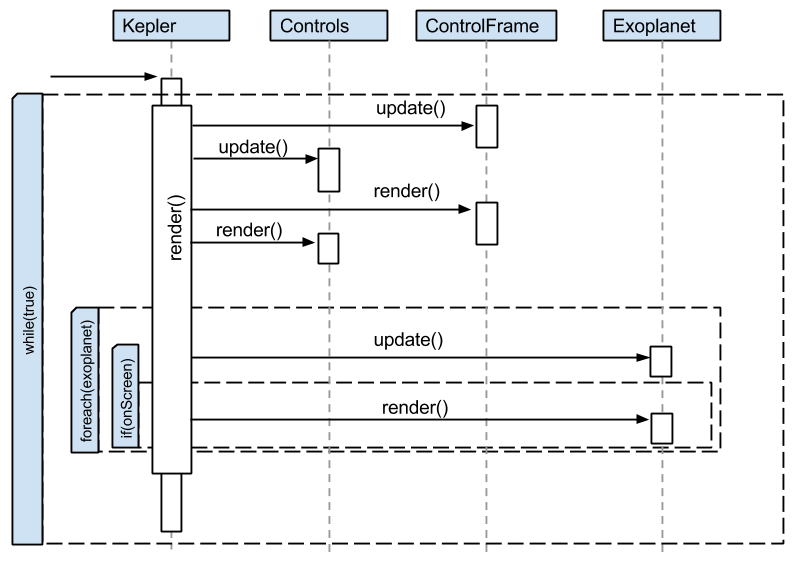
\includegraphics[width=0.8\textwidth]{images/sequence.png}
  \caption{Sequence Diagram of IKVT render cycle}  
\end{figure}

 \item UML Class Diagram
 \\image\\description of\\what it shows about visualisation
 \begin{figure}[H]
  \centering
      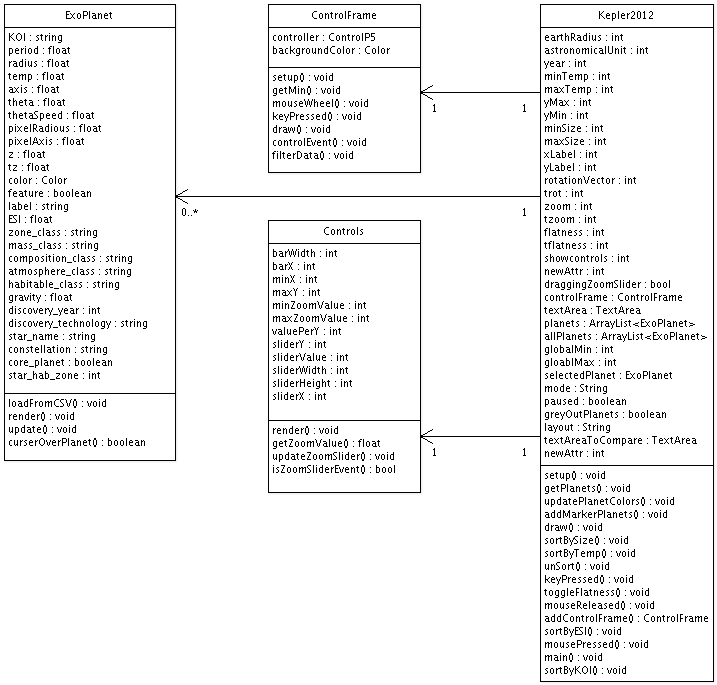
\includegraphics[width=0.8\textwidth]{images/classDiagram.png}
  \caption{Class Diagram of IKVT}  
\end{figure}
 

\end{enumerate}

\section{Visualisation Design}
The requirements produced in the Requirements Analysis chapter provide a
description of the functionality that needs to be designed for this
visualisation. By adding additional details to these requirements we can design
how the visualisation should look, behave, and function.

By using abstract user interface design the layout and configuration of each
element can be
planned and coordinated without the need for excessive details which are likely
to change
throughout the course of the project (e.g. colours and content) \cite{martin}.

\subsection{Functional Requirement}
\begin{enumerate}
{\bf
 \item[R1.] The visualisation needs to display planetary information to convey
knowledge to users.
}

  This requirement needs some form of textual display in order to convey enough
of the information about exoplanets to the user. The most obvious choice for
this would be to use a Java TextArea object to display each of the key
attributes of each Exoplanet. The following figure is a mockup of the text area
showing the information about each planet that will be displayed and the method
calls that will be used.

\begin{figure}[H]
  \centering
      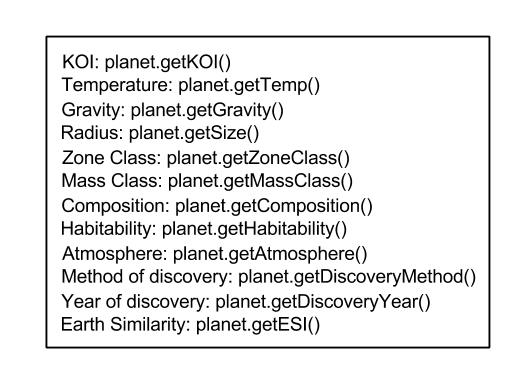
\includegraphics[width=0.8\textwidth]{images/textAreaMockup.png}
  \caption{Mockup of the text area}  
\end{figure}

SELECTIONG ~
All planets need to be selectable and react appropriately when
clicked.

To fulfill this requirement every planet needs to be able to be selected. This
involves detecting when a user clicks and then finding whether any planets are
located in that space. This is more complex in this system as it requires
detecting where each planet is in a 3D space and checking whether the 2D
location of the mouse click coincide. 

When a planet is successfully selected it needs to provide feedback and
information to the user to inform them that it has been selected and also to
provide relevant information.

\begin{figure}[H]
  \centering
      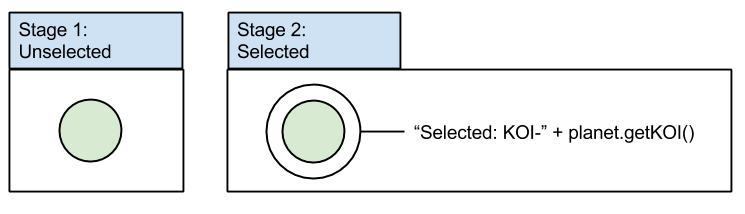
\includegraphics[width=.8\textwidth]{images/mockSelected.png}
  \caption{Mockup selection process}  
\end{figure}

When a planet is selected all other planets in the same solar system
need to become more visible.

When a planet has been successfully selected all of the other planets in the
same solar system (sister planets) need to become highlighted. This can be done
by treating them as if they were selected and providing an additional indication
that they are not actually selected.  
\begin{figure}[H]
  \centering
      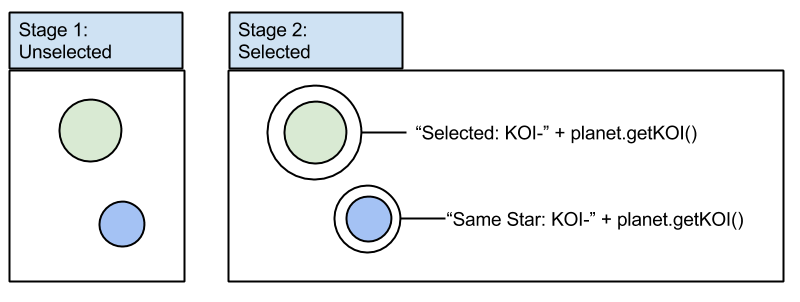
\includegraphics[width=.8\textwidth]{images/selectedSisterPlanets.png}
  \caption{Mockup highlight sister planets process}  
\end{figure}

{\bf
 \item[R2.] The visualisation needs to allow exoplanets to be compared against
one another.}

\begin{figure}[H]
  \centering
      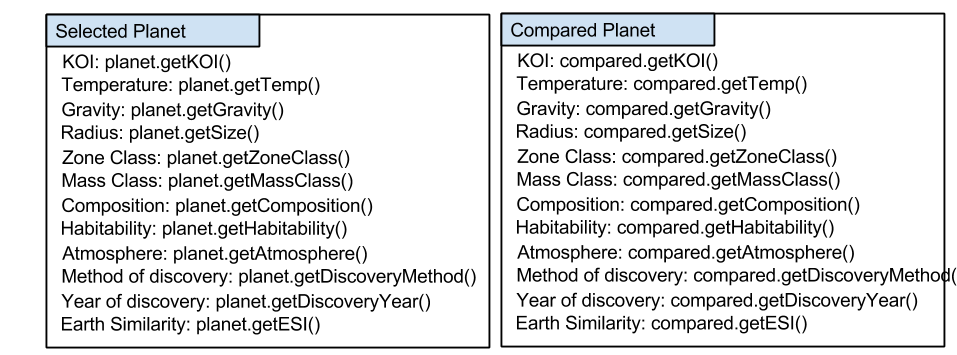
\includegraphics[width=.7\textwidth]{images/mockComparePlanets.png}
  \caption{Mockup compare planets text areas}  
\end{figure}

Using each of the previously discussed elements of interacting with the
visualisation this requirement is fulfilled. The text areas coupled with the
main visualisation window mean that all of the important and valuable
information about each exoplanet can be conveyed to a user.

{\bf
 \item[R3.] The planets need to be able to be ordered by their similarity to
earth (ESI) and by their Kepler Object of Interest number (KOI).}

To fulfill this requirement the visualisation needs to allow users to view the
exoplanets in a way that uses the Earth as a point of reference and their Earth
Similarity Index (ESI) to order them and control their position. The following
figures display an abstract mockup of how this would be done.

\begin{figure}[H]
  \centering
      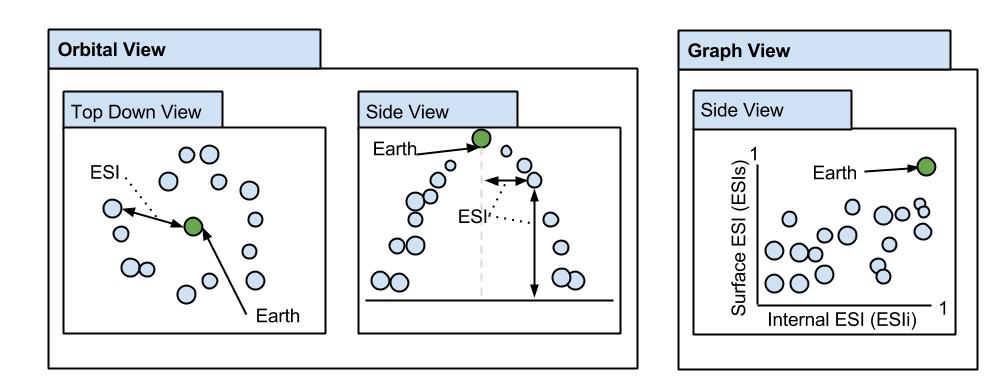
\includegraphics[width=1\textwidth]{images/mockupESI.png}
  \caption{Mockup of ESI views}  
\end{figure}


{\bf
 \item[R4.] The visualisation needs to allow users to define ranges of planetary
attributes to filter which planets are displayed.}

To fulfill this requirement a method of filtering exoplanets by their attributes
in order to control the number and types of planets displayed to the user. A
common method of achieving this is to use a set of sliders that allow a user to
filter something by a set of values. For example in this system a slider could
be used to control the size of planets that are displayed.

\begin{figure}[H]
  \centering
      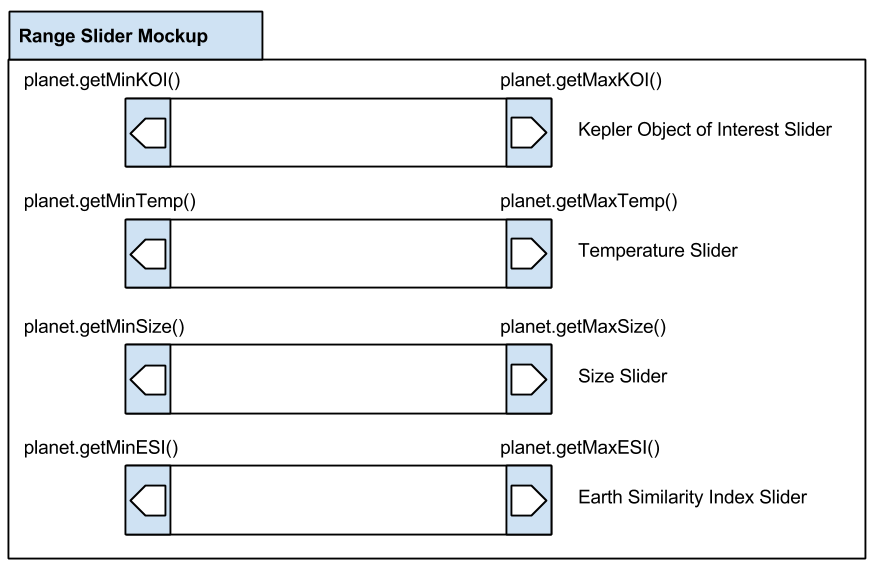
\includegraphics[width=.8\textwidth]{images/mockSlider.png}
  \caption{Mockup of range sliders}  
\end{figure}



{\bf
 \item[R5.] Users need to be able to view the habitable zones of stars in relation to the planets orbiting them.}

\begin{figure}[H]
  \centering
      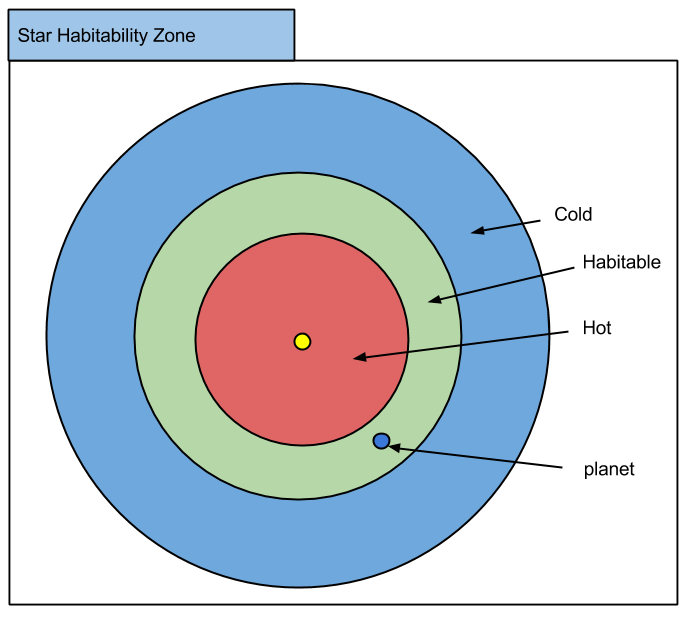
\includegraphics[width=.5\textwidth]{images/mockStarHabitability.png}
  \caption{Mockup star habitability zone}  
\end{figure}




\end{enumerate}

\subsection{Nonfunctional Requirement}

\begin{enumerate}


{\bf \item[R6.] All interaction methods must be visible and intuitive.}
\begin{figure}[H]
  \centering
      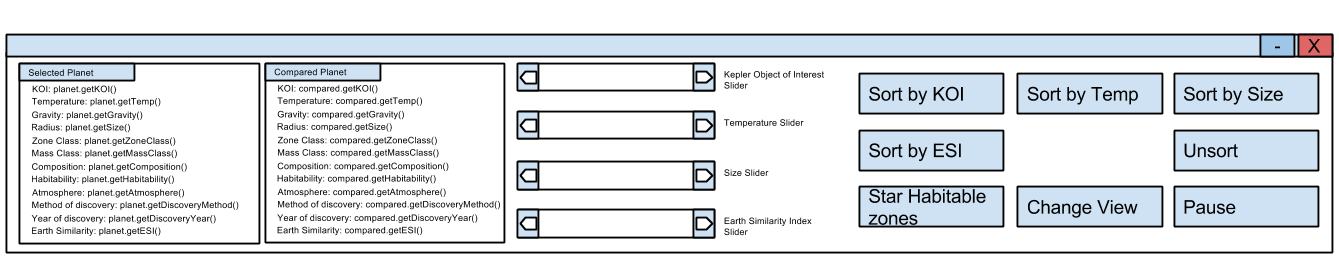
\includegraphics[width=1\textwidth]{images/allTogether.png}
  \caption{Mockup of the interaction panel}  
\end{figure}

 The visualisation needs to have a range of interactive buttons for
each element of interactivity in the system to help inform users how to use the
system.

\begin{figure}[H]
  \centering
      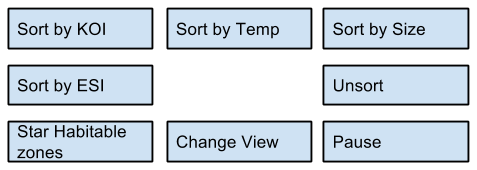
\includegraphics[width=0.5\textwidth]{images/mockButtons.png}
  \caption{Mockup of interactive buttons}  
\end{figure}

{\bf \item[R7.] The visualisation must remain uncluttered.}

By separating each of the interactive components into a separate window inside
the visualisation it provides 

The visualisation must not show so much information that it
causes information overload for users.

The ability to filter and sort the exoplanets gives a user the tools needed to
reduce the quantity of planets displayed in the visualisation and thus the
information load imposed on users. 
In addition to this, by having the text area that displays the information about
selected planets separate from the main visualisation it reduces the cognitive
load on users as they don't have to use this component until they want to. ~


{\bf  \item[R8.] There needs to be two modes of interaction with the system,
keyboard and mouse vs gesture based.}

The above requirements mostly relate to the keyboard an mouse system although some of the requirements do carry through to the Microsoft Kinect system as well. 

For the Kinect system the key difference is that the user will be able to control the main visualisation window with gestures. This means incorporating a means of detecting the gestures. 
\begin{figure}[H]
  \centering
      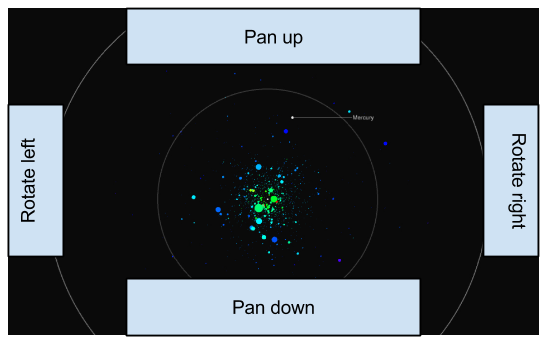
\includegraphics[width=0.7\textwidth]{images/mockKinect.png}
  \caption{Mockup of the Kinect system}  
\end{figure}

As the Kinect sensor no longer requires the use of a mouse the visualisation
design needs to be modified to accommodate the use of gestures. This meant incorporating new cursors to indicate the state of the visualisation.
There are 7 states that the cursor needs to be able to be in to inform the user
of what action they are performing. These states are

\begin{enumerate}
 \item default cursor, hand is at rest
 \item panning up, hand is raised
 \item panning down, hand is lowered
 \item rotating left, hand is to the left
 \item rotating right, hand is to the right
 \item zooming in, hand is pressed forward
 \item zooming out, hand is pulled backwards
\end{enumerate}
\begin{figure}[H]
  \centering
      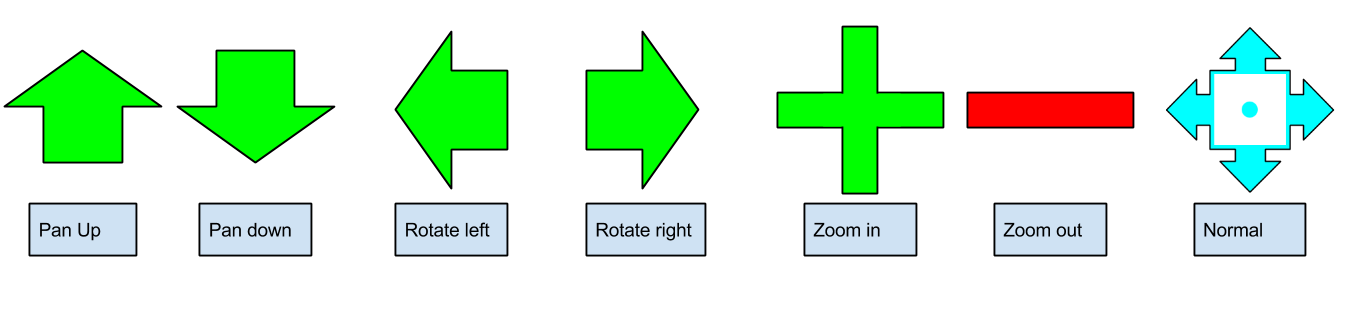
\includegraphics[width=0.9\textwidth]{images/curserImages.png}
  \caption{Mockup of cursor images for Kinect system}  
\end{figure}

Having a range of icons that clearly display these states is vital for keeping
the user informed of what they are doing. The icons designed for this purpose
are in the following figure

\begin{figure}[H]
  \centering
  ~
      %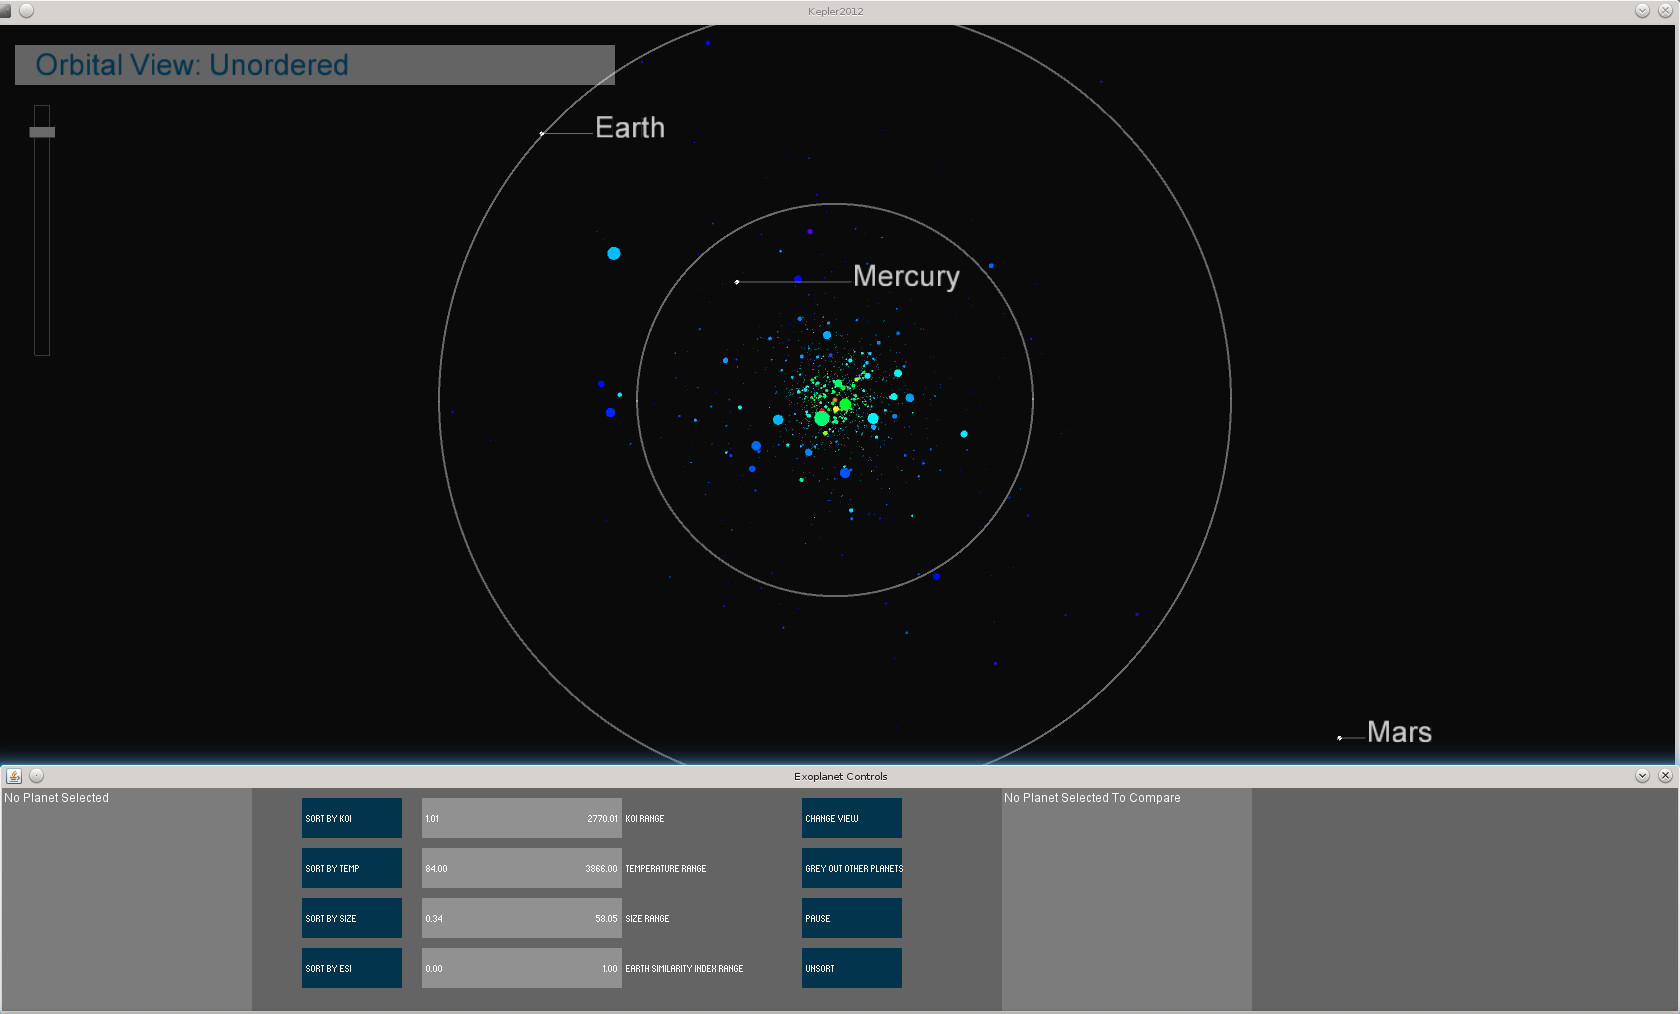
\includegraphics[width=0.8\textwidth]{images/layout_horizontal.jpg}
  \caption{Cursors for Kinect sensor}  
\end{figure}


\end{enumerate}


